\section{Results}
\label{sec:results}

\subsection{Local data structure}
\label{sec:data_structure}

The local fallback dataset covered a broad range of mixture quantities and curing ages (Table~\ref{tab:dataset-summary}). Cement had the strongest absolute target correlation in the generated registry candidates, with a correlation of 0.822. This statement is limited to the current fallback data and should be mapped to the numerical registry before final release.

\begin{figure}[htbp]
\centering
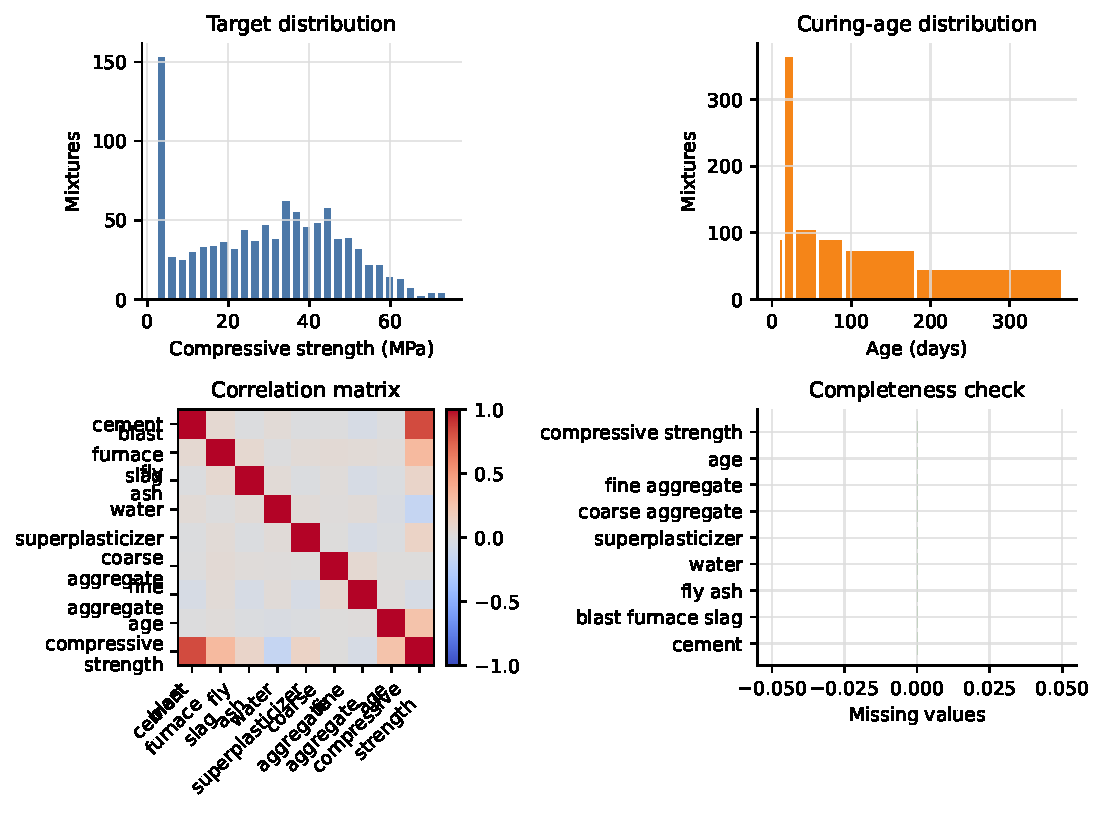
\includegraphics[width=0.95\linewidth]{figures/fig_dataset_overview.pdf}
\caption{Overview of the local concrete-strength fallback dataset used in the demonstration. The source label for the generated artifacts is \texttt{DETERMINISTIC\_FALLBACK\_NOT\_UCI}.}
\label{fig:dataset-overview}
\end{figure}

\subsection{Predictive performance}
\label{sec:predictive_performance}

The selected standardized ridge model achieved a test RMSE of 6.234~MPa, MAE of 4.964~MPa, \(R^2 = 0.886\), and bias of 0.032~MPa (Table~\ref{tab:model-performance}). The standardized ordinary least-squares comparator gave nearly identical test metrics in this generated run. Both linear models improved substantially over the training-mean baseline, which had a test RMSE of 18.447~MPa and \(R^2=-0.002\). The near equality of the ordinary least-squares and ridge results indicates that the selected ridge penalty primarily functions as a conservative regularization choice in this demonstration rather than producing a distinct accuracy gain.

\begin{table}
\caption{Train and test performance for baseline, ordinary least squares, and ridge models. Error and bias values are in MPa.}
\label{tab:model-performance}
\begin{tabular}{llrrrrr}
\toprule
Model & Alpha & Train RMSE (MPa) & Test RMSE (MPa) & Test MAE (MPa) & Test R2 & Test Bias (MPa) \\
\midrule
Training-mean baseline & -- & 18.115 & 18.447 & 15.525 & -0.002 & -0.740 \\
Standardized OLS & 0.000 & 6.366 & 6.234 & 4.964 & 0.886 & 0.033 \\
Standardized ridge & 1.000 & 6.366 & 6.234 & 4.964 & 0.886 & 0.032 \\
\bottomrule
\end{tabular}
\end{table}


\begin{figure}[htbp]
\centering
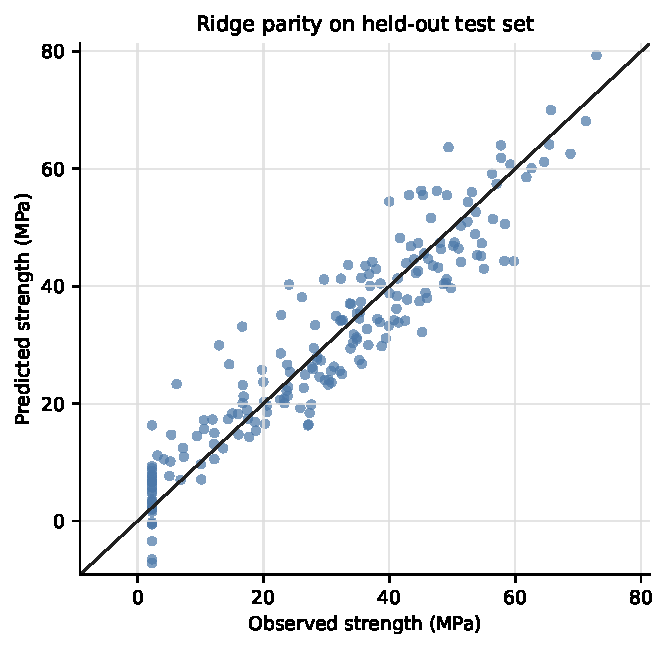
\includegraphics[width=0.78\linewidth]{figures/fig_parity_ridge.pdf}
\caption{Observed versus predicted compressive strength for the selected ridge model on the held-out fallback test set.}
\label{fig:parity-ridge}
\end{figure}

\subsection{Residual and age-stratified error patterns}
\label{sec:error_patterns}

The residual diagnostic plot showed the distribution of ridge prediction errors across predicted strength values (Figure~\ref{fig:residuals}). Age-stratified metrics indicated larger MAE in the youngest and oldest age groups than in the 8--28 day and 29--90 day groups (Table~\ref{tab:error-by-age}). In particular, the \(>90\)-day group contained 19 test observations and had an MAE of 6.572~MPa. Because these bins come from the local fallback split, they should be interpreted as diagnostic summaries rather than population-level evidence.

\begin{figure}[htbp]
\centering
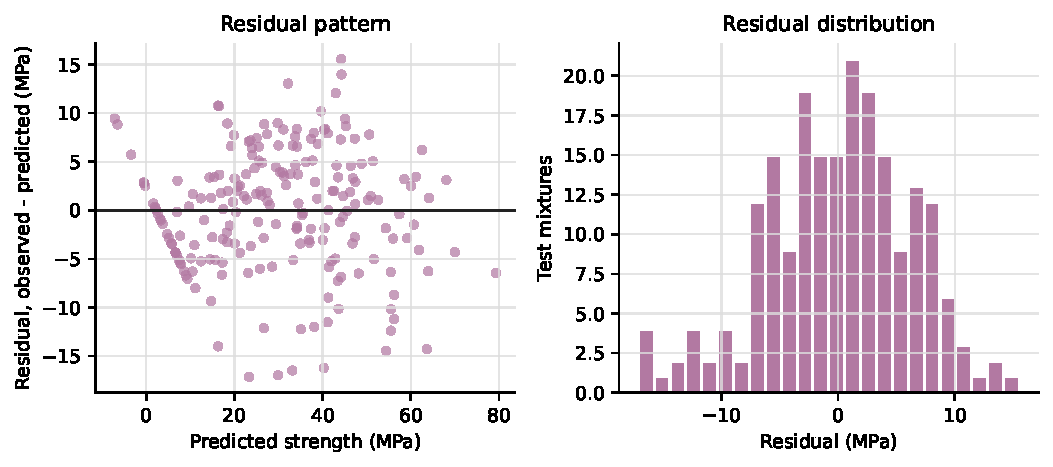
\includegraphics[width=0.78\linewidth]{figures/fig_residuals.pdf}
\caption{Residual diagnostics for the selected ridge model on the held-out fallback test set. Residual summaries are descriptive and do not establish validity for the official UCI observations.}
\label{fig:residuals}
\end{figure}

\begin{table}
\caption{Ridge-model test-set error stratified by curing-age group. Error and strength values are in MPa.}
\label{tab:error-by-age}
\begin{tabular}{lrrrrr}
\toprule
Age bin & N & Mean age (days) & MAE (MPa) & Bias (MPa) & Mean strength (MPa) \\
\midrule
<=7 days & 63 & 4.937 & 5.650 & 3.102 & 21.709 \\
8-28 days & 79 & 25.342 & 4.225 & -0.420 & 29.903 \\
29-90 days & 45 & 72.622 & 4.622 & -3.227 & 34.183 \\
>90 days & 19 & 246.579 & 6.572 & -0.552 & 49.178 \\
\bottomrule
\end{tabular}
\end{table}


\begin{figure}[htbp]
\centering
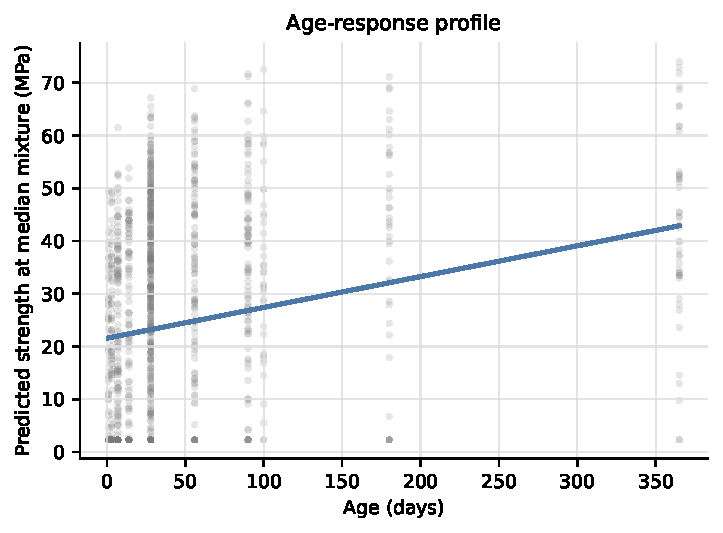
\includegraphics[width=0.78\linewidth]{figures/fig_age_response.pdf}
\caption{Generated age-response diagnostic for the selected ridge workflow. The display is used to inspect the local fallback data and should not be generalized beyond that provenance.}
\label{fig:age-response}
\end{figure}

\subsection{Coefficient and ablation diagnostics}
\label{sec:coefficients_ablation}

The coefficient figure summarizes the standardized ridge coefficients for the eight predictors (Figure~\ref{fig:coefficients}). These coefficients describe conditional linear associations after standardization and shrinkage; they are not direct physical effect sizes. In the single-feature ablation analysis, removing cement produced the largest RMSE increase, from 6.234~MPa to 16.191~MPa, for a delta of 9.958~MPa (Table~\ref{tab:ablation}). Removing blast-furnace slag and age also increased RMSE by more than 1~MPa. The small negative delta for coarse aggregate means that this particular ablation run produced a slightly lower test RMSE after removing that feature; it should not be overinterpreted.

\begin{figure}[htbp]
\centering
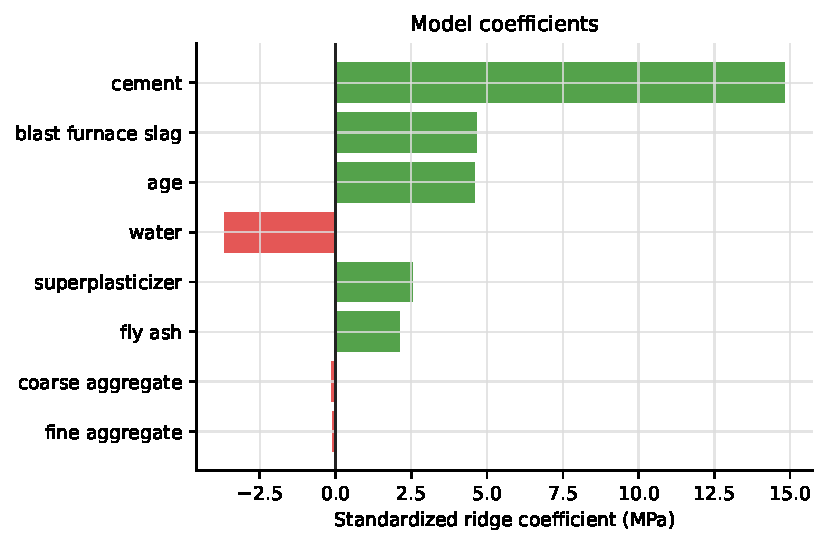
\includegraphics[width=0.78\linewidth]{figures/fig_coefficients.pdf}
\caption{Standardized ridge coefficients for the selected model. Coefficients are model diagnostics for the local fallback data rather than causal estimates.}
\label{fig:coefficients}
\end{figure}

\begin{table}
\caption{Single-feature ablation using the selected ridge penalty. RMSE values are in MPa.}
\label{tab:ablation}
\begin{tabular}{lrr}
\toprule
Removed feature & Test RMSE (MPa) & Delta RMSE (MPa) \\
\midrule
cement & 16.191 & 9.958 \\
blast furnace slag & 7.749 & 1.515 \\
age & 7.735 & 1.502 \\
water & 6.834 & 0.601 \\
fly ash & 6.492 & 0.258 \\
superplasticizer & 6.460 & 0.227 \\
fine aggregate & 6.236 & 0.002 \\
coarse aggregate & 6.221 & -0.013 \\
\bottomrule
\end{tabular}
\end{table}

